\documentclass[aspectratio=169]{beamer}

\usepackage{tikzlings}

\setbeamertemplate{navigation symbols}{}
\setbeamertemplate{background canvas}{%
\begin{tikzpicture}[remember picture,overlay]
\node at (current page.center){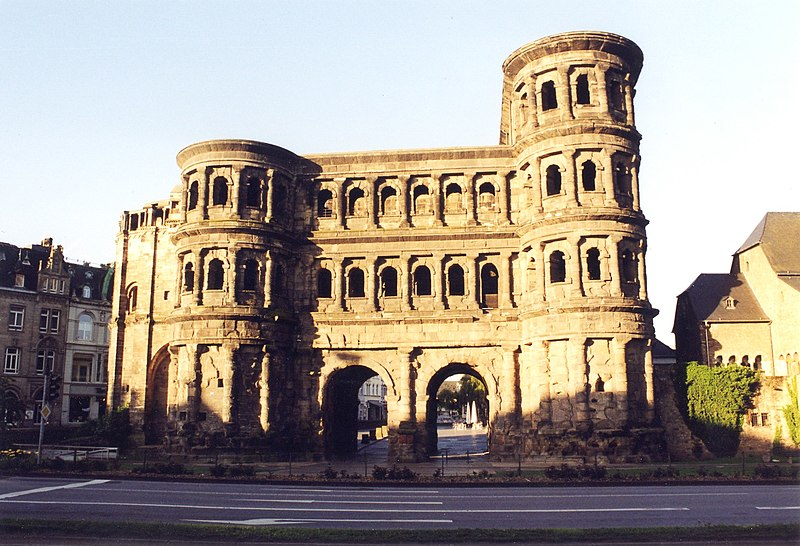
\includegraphics[width=\paperwidth]{Porta_Nigra}};
\end{tikzpicture}}

% trick taken from https://topanswers.xyz/tex?q=1989
\tikzset{
    use page relative coordinates/.style={
        shift={(current page.south west)},
        x={(current page.south east)},
        y={(current page.north west)}
    },
}

\makeatletter
\newcommand*{\overlaynumber}{\number\beamer@slideinframe} 
\makeatother

\begin{document}

\def\stepnumber{700}
\begin{frame}<0>[label=porta]
  \begin{tikzpicture}[remember picture, overlay,use page relative coordinates]
    \node[xscale=-1,scale=0.2+\overlaynumber*1.4/\stepnumber] at (0.44-\overlaynumber*0.25/\stepnumber,0.15+\overlaynumber*0.12/\stepnumber) {
\includegraphics{roman_bear}};
    \node[xscale=-1,scale=0.2+\overlaynumber*1.4/\stepnumber] at (0.47-\overlaynumber*0.07/\stepnumber,0.15+\overlaynumber*0.12/\stepnumber) {
\includegraphics{roman_bear}};
    \node[scale=0.2+\overlaynumber*1.4/\stepnumber] at (0.56+\overlaynumber*0.07/\stepnumber,0.15+\overlaynumber*0.12/\stepnumber) {
\includegraphics{roman_bear}};
    \node[scale=0.2+\overlaynumber*1.4/\stepnumber] at (0.59+\overlaynumber*0.25/\stepnumber,0.15+\overlaynumber*0.12/\stepnumber) {
\includegraphics{roman_bear}};
    
    % credit for background image
    \node[white,text width=.7\paperwidth,font=\tiny,align=center] at ([yshift=0.35cm]current page.south) {Image source: \url{https://commons.wikimedia.org/wiki/File:Porta_Nigra_Landseite.jpg}};  
 
  \end{tikzpicture}
  \pause[\stepnumber]
\end{frame}	

\foreach \macro in {0,...,100}{\againframe<1>{porta}}
	
\againframe{porta} 
  
\foreach \macro in {0,...,50}{\againframe<\stepnumber>{porta}}  

\end{document}